\documentclass[a4paper]{article}
\usepackage{fontspec}
\usepackage{amsmath}
\usepackage{amssymb}


%%%%lualatex on
%\usepackage{luatextra}
%Ligatures={Contextual, Common, Historical, Rare, Discretionary}
%\setmainfont[Mapping=tex-text]{Linux Libertine O}

\usepackage{natbib}

\title{Note about WSC}
\author{Simon}
\begin{document}
\maketitle
\section{Classic Cultural Evolution}



The cultural evolution's literature gives us a way to interpret evolution of cultural artifact such as those produce in economical field. We want to confront well know cultural evolution's mechanism to well known economical evolution's mechanism and see and show their differences.

\subsection{Verification}
First we verify that our model implements well the already known cultural evolution mechanisms.

Here we follow \cite{mesoudi2009randomcopyingfrequencydependencopyingandulturechange,bentley2004randomdriftandculturechange} and look for the evolution of a single traits depending on the innovation rate $\mu$ in a 250 agents population during 1000 steps.


With infinite innovation possibilities(ie : $n$ variant $| n\in\mathbb{A} $) the results, showed in the figure \ref{fig:allMutation} are the same that those from \cite{bentley2004randomdriftandculturechange}.
\begin{figure}[hbp]
	\begin{center}
		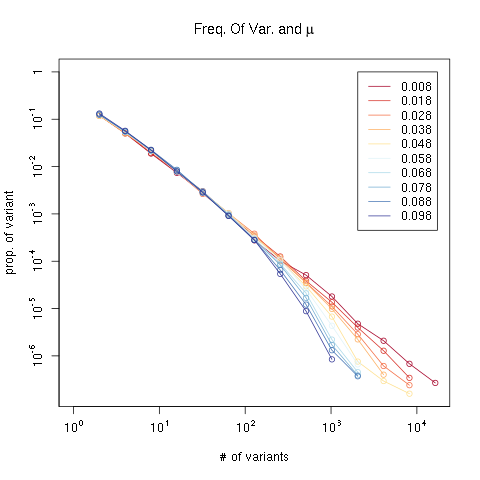
\includegraphics[width=7cm]{img/allmuRandMax.png}
	\end{center}
	\caption{rand()\%RAND\_MAX}
	\label{fig:allMutation}
\end{figure}

\subsection{generalisation: Multiple Traits (all varying on $\mathbb{N}$)}
Once the results are verified, we generalized those result for $n$ possible traits.

In that case individual owns a vector of $n$ traits. One a cultural exchange occurs the whole vector is exchanged.

Individual carries multiples traits (ie price in our experiment), we check that it does not change the result of the algorithm in the long terms, each traits will evolve following the same curves than when just one trait is evolving. The results are shown in figures \ref{fig:10resources}. Those results are statistically the same than those from the previous experiments.
\begin{figure}[h]
	\begin{center}
		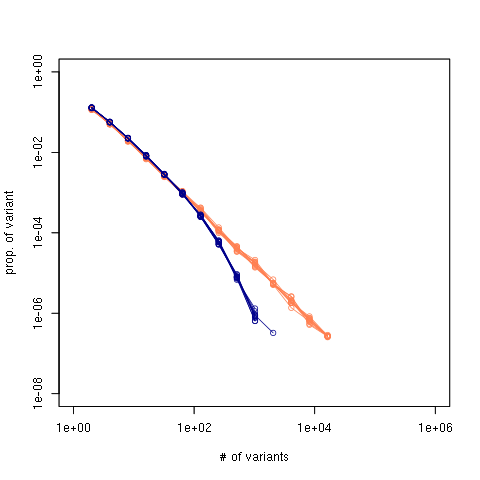
\includegraphics[width=6cm]{img/10resources.png}
	\end{center}
	\caption{$\mu=\{.08,.098\}$ for 10 resources}
	\label{fig:10resources}
\end{figure}


\section{Cultural Mechanisms Comparison}

Now that we have shown our model reproduce well known cultural evolution mechansims we will compare the evolution of the system when it is submit to the previous mechanism studied to the evolution of the same system submitted to the mechanisms cultural transmission and innovation used by \cite{gintis2006theemergenceofapricesystemfromdecentralizedbilateralexchange}.

\subsection{framework Adjustment}
In order to allow such comparison we will do our simulation using the same parameters used by Gintis which are : a population with 100 agents per good assuming six good so 600 agents evolving during 1500 steps and with a innovation rate of .01.

It worth to notice here than the way Gintis counts the steps is slightly different than the others article. Indeed in Gintis agents follow 10 Produce/Trade/Consume cycles before exchanging their cultural belief, which means than when in the previous runs we speak about 5 runs, it means in Gintis framework ``5 cycle of cultural exchange'' so 50 steps.

The results are those expected : given the much higher number of agents and 


\subsection{Comparison}
In order to compare the different mechanisms used in the different paper we will cross them  following the table \ref{tab:exp}.
\begin{table}
	\centering
	\begin{tabular}{l|c|c}
		& Rand & Gintis \\\hline
		$\mu$ &A & B \\
		$\mu +\alpha$ & C & D \\
	\end{tabular}
	\caption{Experimental Setup}
	\label{tab:exp}
\end{table}


First we check how those different mechanisms impact the power law distribution.

\begin{figure}[hbp]
	\begin{center}
		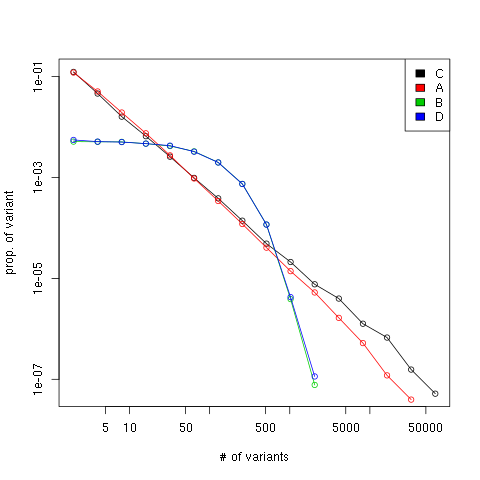
\includegraphics[width=6cm]{img/powerABCD.png}
	\end{center}
	\caption{power law for each exp define in table \ref{tab:exp} after 2000 step}
	\label{fig:powerABCD}
\end{figure}

As expected depending on the selection process the repartition follow a power law (random selection) or a exponential law).

Next let's have a look which combination lead to the right economical processes.

\begin{table}
	\centering
	\begin{tabular}{l c c}
		& Random Transmission & Gintis Transmission \\
		FRI & \raisebox{-.5\height}{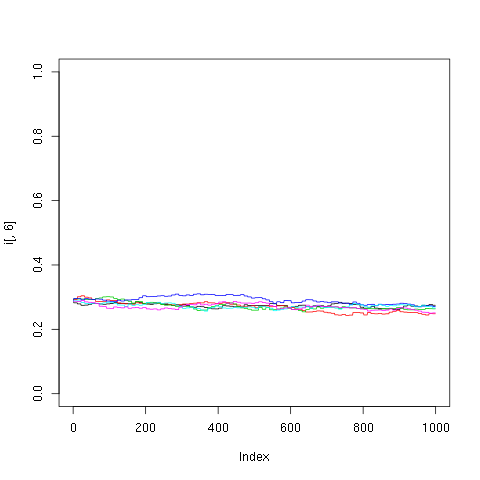
\includegraphics[width=5cm]{img/sdEvolEXP2.png}}&\raisebox{-.5\height}{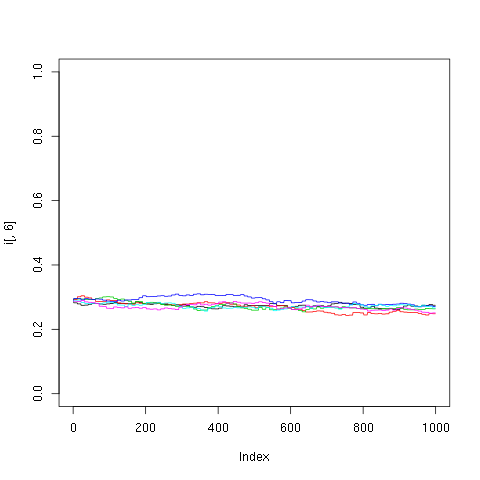
\includegraphics[width=5cm]{img/sdEvolEXP2.png}} \\
		GRI & \raisebox{-.5\height}{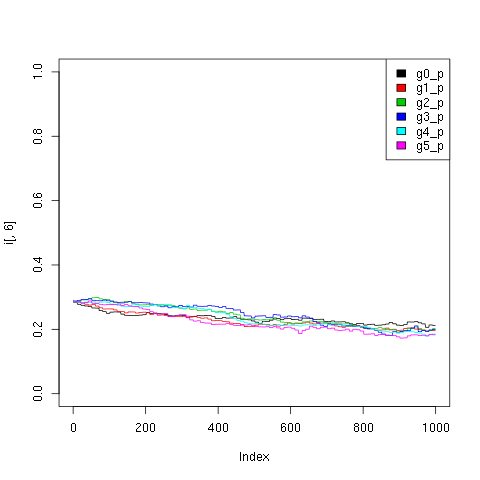
\includegraphics[width=5cm]{img/sdEvolEXP3.png}}&\raisebox{-.5\height}{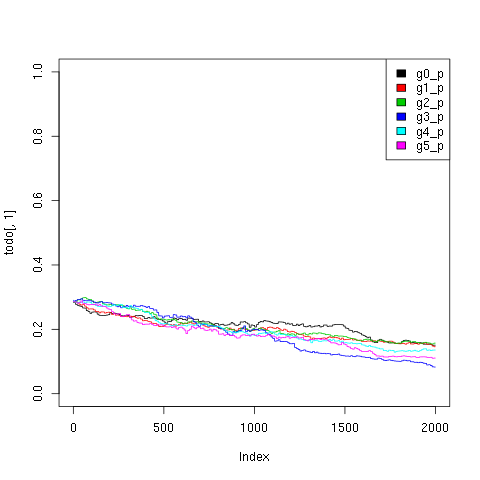
\includegraphics[width=5cm]{img/sdEvolEXP4.png}}

	\end{tabular}
	\caption{Evolution of SD. FRI : Fully Random Innovation, GRI: Gintis Random Innovation}
	\label{tab:sdevol}
\end{table}

\section{Other reflexion}
\subsection{Discrete and finite inovation space}
The Finite Innovation Effect (ie : $n$ variant  $| n\in\{0,\cdots,100\}$). If choose a innovation mechanism such as the number of possible new variant is finite, we see a strange ``anticonformist-like'' effect such the one shown by \cite{mesoudi2009randomcopyingfrequencydependencopyingandulturechange}. This effect is visible in the figure \ref{fig:finitEffect}.
\begin{figure}[h]
	\begin{center}
		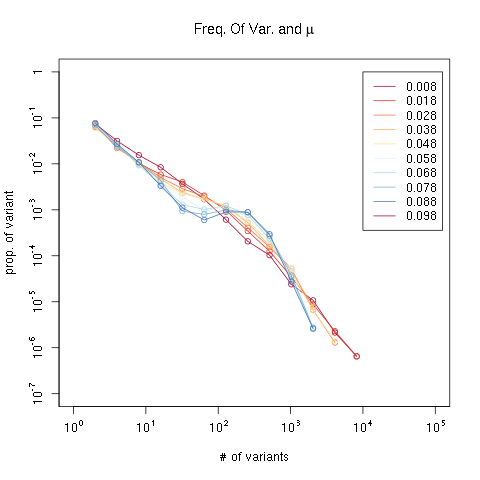
\includegraphics[width=7cm]{img/allmu.png}
	\end{center}
	\caption{rand()\%100}
	\label{fig:finitEffect}
\end{figure}

\subsection{Validation of the curves similarities}
\begin{figure}[h]
	\begin{center}
		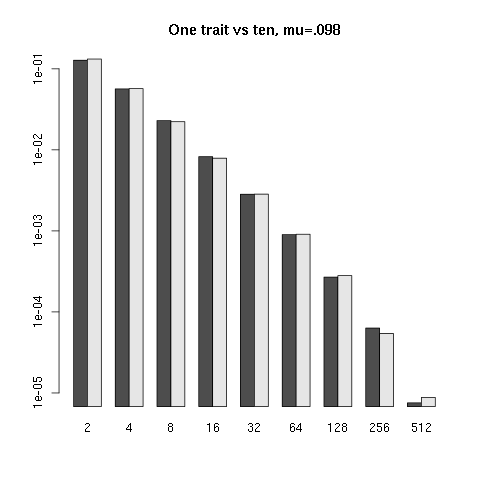
\includegraphics[width=6cm]{img/OneVsTenMu098.png}
		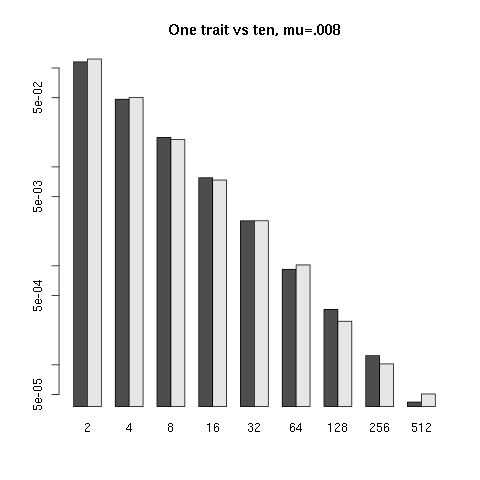
\includegraphics[width=6cm]{img/OneVsTenMu008.png}
	\end{center}
	\caption{$\mu=\{.08,.098\}$ for one of the 10 resources VS one only}
	\label{fig:OneVsTen}
\end{figure}
\bibliographystyle{apalike}
\bibliography{/home/scarrign/Documents/biblio/bib/phd.bib}  
\end{document}


